ALICE computing framework. \subsection{The ALICE High Level Trigger}

The HLT is a software-based data processing system tasked with the filtering of events from the CTS and the reduction of event data volume. This system is shown within the context of the ALICE dataflow in Figure~\ref{alice-hlt-diagram}. Related tasks such as event reconstruction and calibration are also performed by the HLT. The HLT is implemented on 180 computing nodes, with 66 Front-End Processor (FEP) nodes dedicated to input and 8 HLT Output (HLTOUT) nodes dedicated to output. Data processed by the HLT is then stored for offline analysis. The HLT farm is also made available opportunistically to the Worldwide LHC Computing Grid. 

\begin{figure}[h!]
    \centering
    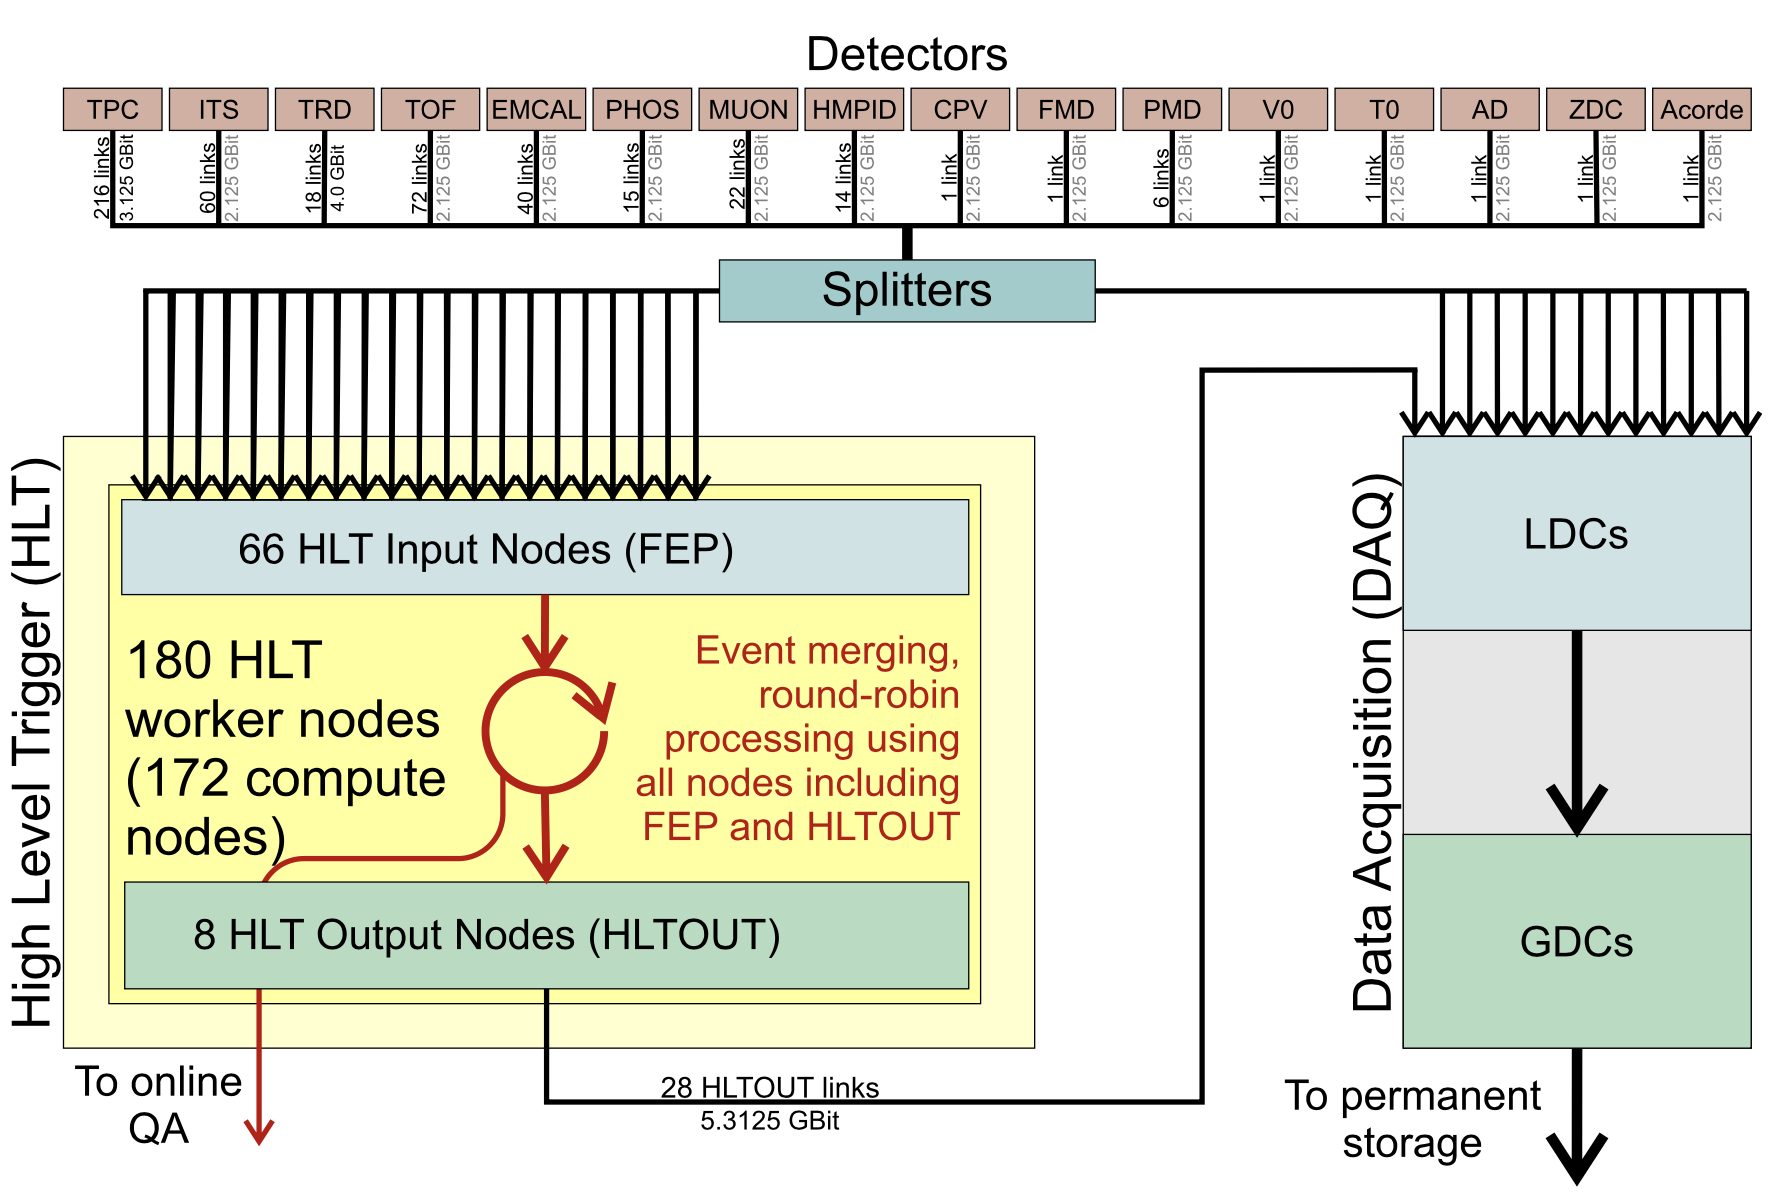
\includegraphics[width=0.7\linewidth]{images/alice/alice-hlt-schematic.png}
    \caption{Schematic of the ALICE trigger and data acquisition systems \cite{alice-rta-trigger}. The HLT receives copies of detector readout data.}
    \label{alice-hlt-diagram}
\end{figure}
 
FEP nodes handle the receipt of detector readout; each FEP node is equipped with a Common FPGA-based Read-Out Receiver Card (C-RORC) which receives data from up to 12 optical data links and streams this data to the RAM of the node machine. The C-RORC takes further advantage of its FPGA architecture by also performing TPC cluster finding, dicussed further in Section~\ref{alice-accel}. The raw detector readout data is then distributed amongst all 180 nodes for further processing.

The HLT processing chain performed on the compute nodes is a publisher-subscriber processing pipeline in which the reconstruction tasks of each subdetector are interwoven. These tasks generally begin with clustering, then developing to track finding and finally the collection of tracks to form events. Monitoring and calibration objects are also produced and saved alongside events. Transport of data to/from the HLT processing chain is built around three pillars:
\begin{itemize}
    \item A primary reconstruction chain receives and sends data, processing events synchronously.
    \item Monitoring side chains run alongside the main chain, subscribing to main chain outputs to avoid disruption.
    \item An additional chain, introduced in Run 2, receives reconstructed events from the output of the main chain to be processed further asynchronously (e.g. for calibration and monitoring).
\end{itemize}
Much of the HLT processing is only possible due to significant upgrades to the ALICE computing framework, culminating in the Online-Offline \cite{alice-o2-tdr} framework.

\subsubsection{Hardware acceleration of the High Level Trigger}
\label{alice-accel}

Many data processing tasks of the ALICE HLT are accelerated by the use of heterogeneous architectures. The TPC cluster finding algorithm is one of many examples of a reconstruction algorithm in the HLT designed with such acceleration in mind. Each particles passing through the TPC leaves a small cluster of signal \say{hits} on each readout plane of the TPC. The cluster finding algorithm calibrates the raw readout, calculates the weighted mean of signals in each plane and merges neighbouring signals in the plane to produce a cluster. Whilst individually this is relatively trivial, high multiplicity makes cluster finding more difficult. This algorithm is however highly parallelisable, with the three steps forming an independent pipeline which can be run separately for separate clusters, and is hence well suited to deployment on FPGAs. Online FPGA processing of TPC clusters is significantly faster than offline on CPUs, as shown in Figure~\ref{alice-fpga-plot}, whilst retaining effectively offline-quality of clustering.

The forming of tracks from TPC clusters is performed by two algorithms, one offline and one online in the HLT. The latter of these benefits from hardware acceleration, using GPU resources in the HLT farm to accelerate track reconstruction. The HLT track reconstruction algorithm uses a cellular automaton to determine candidate trajectories which are then fit with a Kalman filter to construct a track. This is also a highly parallelisable problem, though more computationally intensive than cluster finding. As such, GPUs are well-suited to performing track finding online. Implementing the above algorithm on GPUs thus provides a significant speedup, particularly in cluster-dense environments, as demonstrated in Figure~\ref{alice-gpu-track}.

\begin{figure}[h!]
    \centering
    \begin{subfigure}[b]{0.445\linewidth}
        \centering
        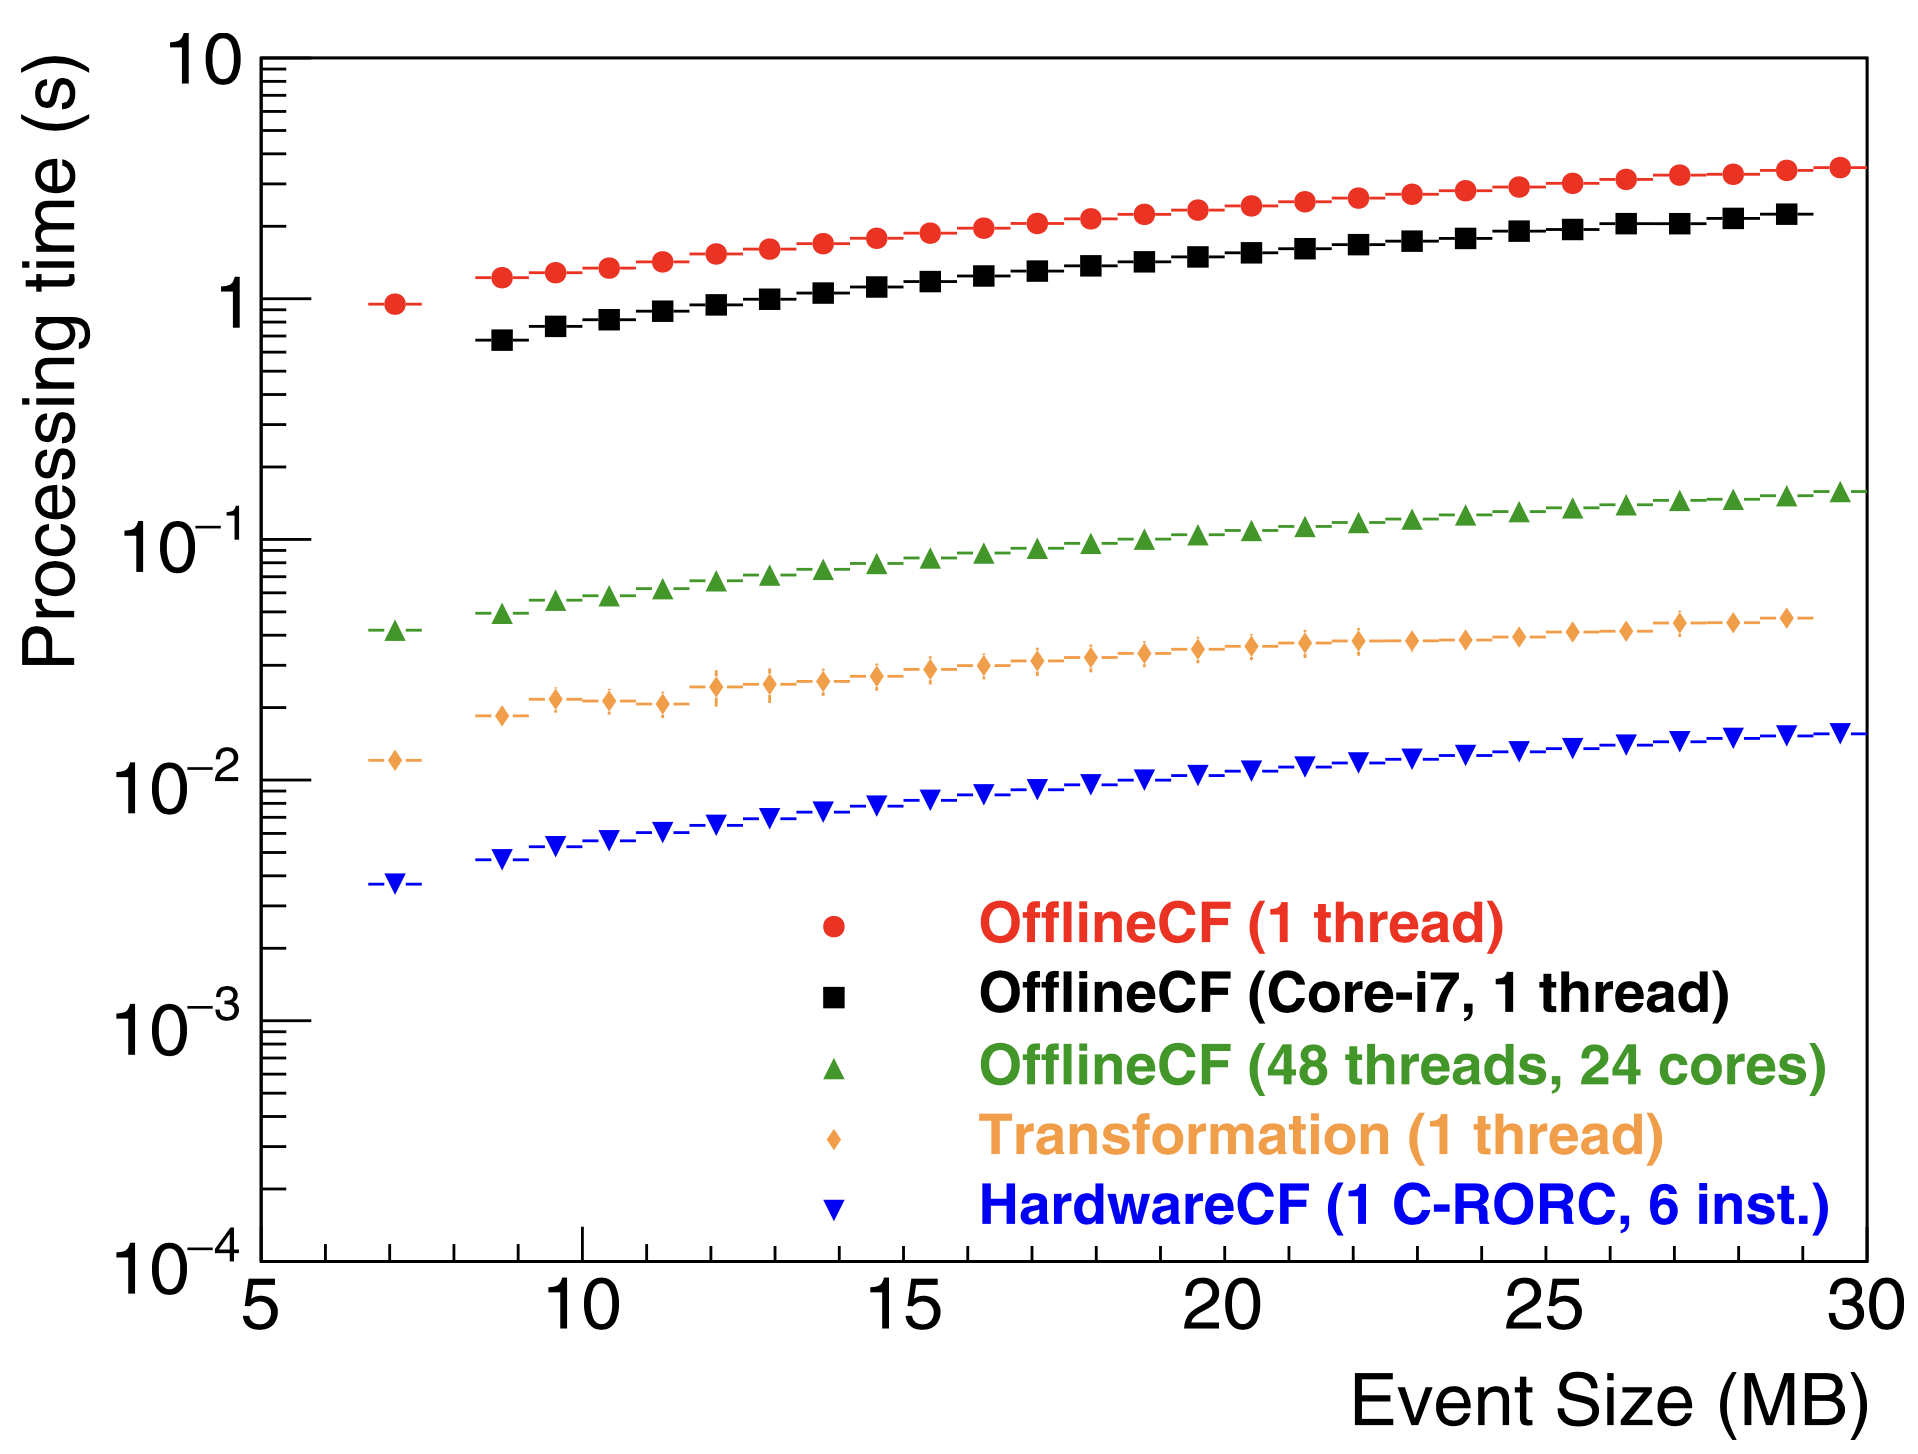
\includegraphics[width=\linewidth]{images/alice/alice-fpga-cluster.png}
        \caption{Implementations of TPC cluster finding~\cite{alice-trigger-run3}. HardwareCF is implemented on C-RORC FPGAs.}
        \label{alice-fpga-plot}
    \end{subfigure}
    \begin{subfigure}[b]{0.505\linewidth}
        \centering
        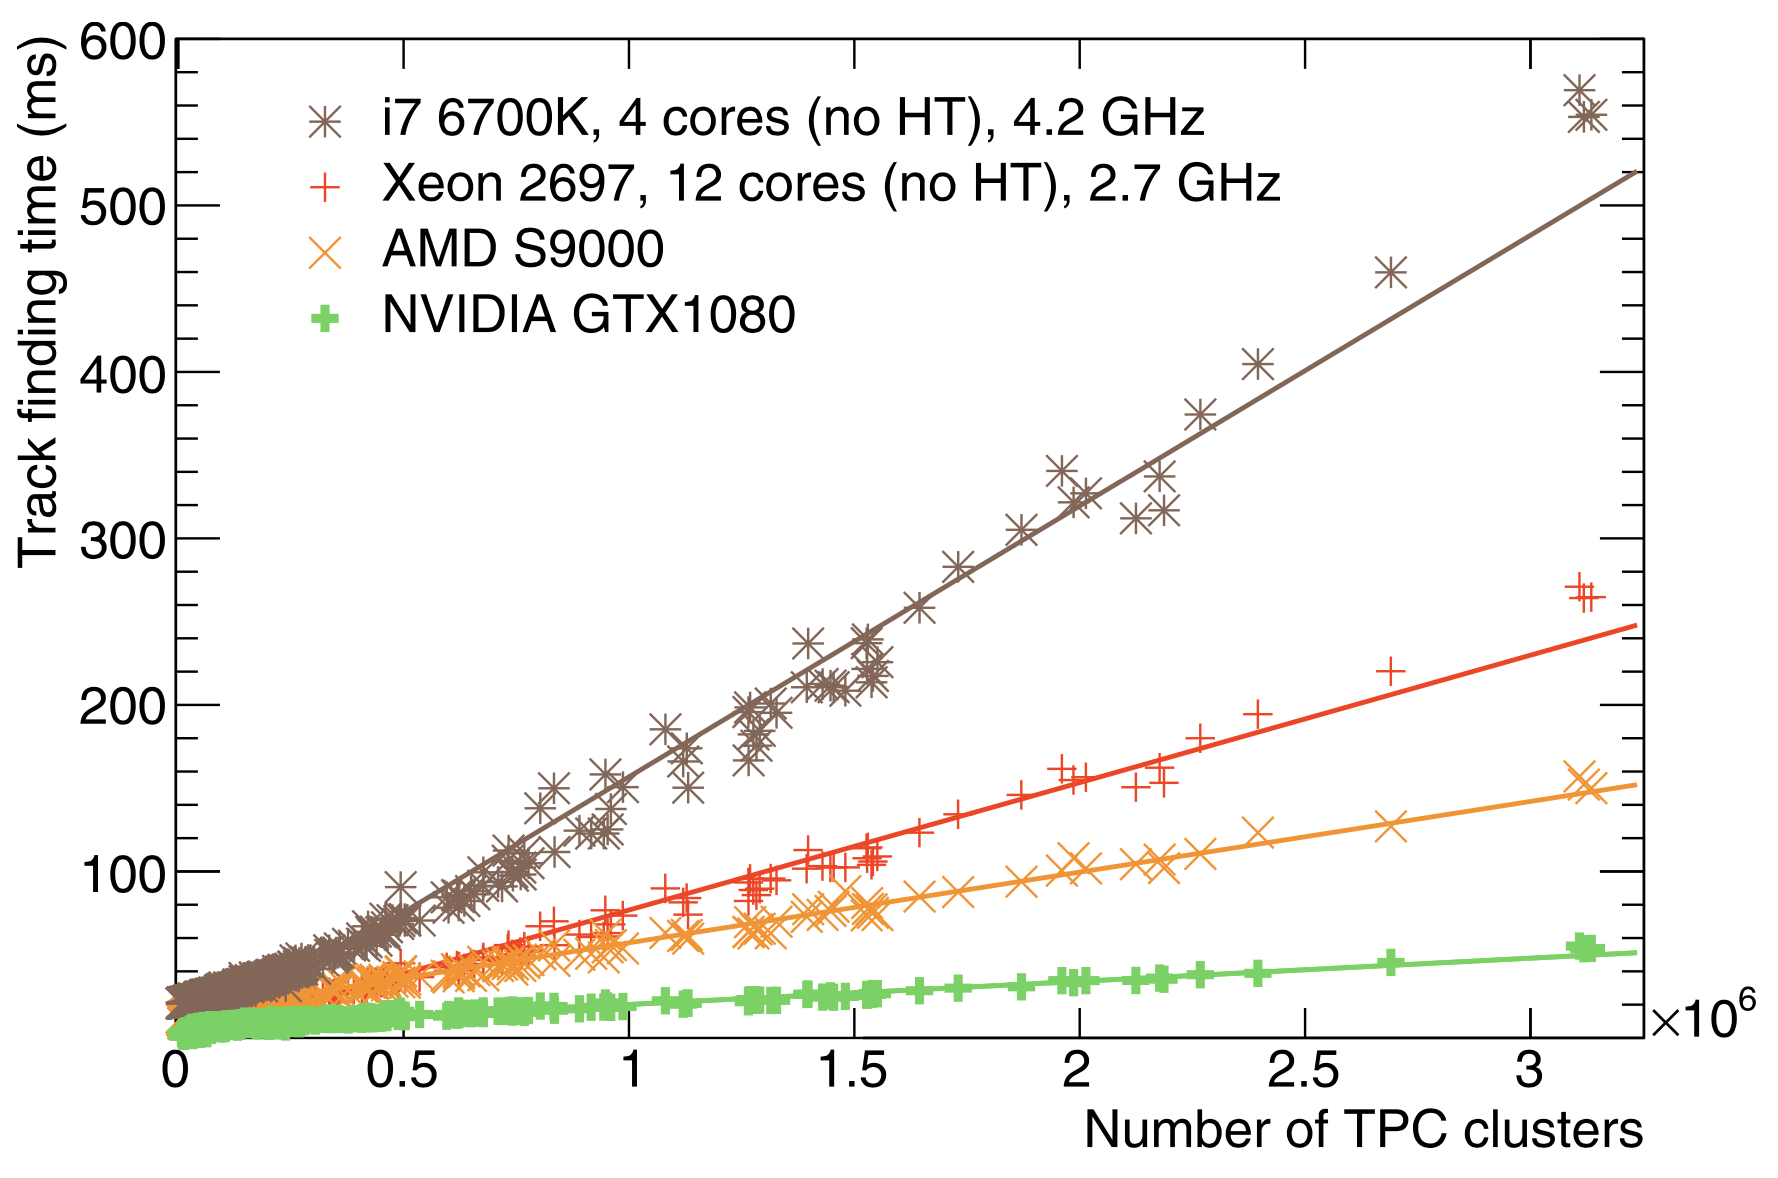
\includegraphics[width=\linewidth]{images/alice/alice-gpu-track.png}
        \caption{Implementations of TPC track finding~\cite{alice-trigger-run3}. Fastest performance achieved with GPU implementation on NVIDIA GTX1080.}
        \label{alice-gpu-track}
    \end{subfigure}
    \caption{Examples of hardware acceleration in ALICE track reconstruction algorithms.}
\end{figure}

\subsubsection{Online calibration of the ALICE Time Projection Chamber}
\label{alice-tpc}
